\documentclass[a4paper,11pt]{jsarticle}


\usepackage{amsmath,amsthm,amsfonts,float,cases,bm,amssymb,amssymb,ascmac,url,color}
\usepackage[dvipdfmx]{graphicx}
\usepackage[all]{xy}
\usepackage{makeidx}
\usepackage[bbgreekl]{mathbbol}
\usepackage[%
 dvipdfmx,% 欧文ではコメントアウトする
 setpagesize=false,%
 bookmarks=true,%
 bookmarksdepth=tocdepth,%
 bookmarksnumbered=true,%
 colorlinks=false,%
 pdftitle={},%
 pdfsubject={},%
 pdfauthor={},%
 pdfkeywords={}%
]{hyperref}
% PDFのしおり機能の日本語文字化けを防ぐ((u)pLaTeXのときのみかく)
\usepackage{pxjahyper}
\DeclareMathSymbol{\bbepsilon}{\mathord}{bbold}{"0F}


\makeindex

\setlength{\textwidth}{\fullwidth}
\setlength{\textheight}{40\baselineskip}
\addtolength{\textheight}{\topskip}
\setlength{\voffset}{-0.55in}

\theoremstyle{definition}
\newtheorem{thm}{定理}[section]
\newtheorem{prop}[thm]{命題}
\newtheorem{cor}[thm]{系}
\newtheorem{dfn}[thm]{定義}
\newtheorem{lem}[thm]{補題}
\newtheorem{rem}[thm]{注意}
\newtheorem{eg}[thm]{例}

\DeclareMathOperator{\Hom}{\mathrm{Hom}}
\DeclareMathOperator{\id}{\mathrm{id}}
\DeclareMathOperator{\Int}{\mathrm{Int}}

\setcounter{tocdepth}{3}%目次に表示する数字の深さ
\setcounter{section}{-1}

\begin{document}
\date{}
\title{ホモトピー論の基本について}

\maketitle

\begin{abstract}
  ホモトピー論の基本について網羅的に書いたものではなく,勉強中に特に注意して考えたことをまとめたもの.構成は\cite{fomenko2016homotopical}\cite{whitehead2012elements}に依る.
\end{abstract}

\tableofcontents

%section 1
\section{準備}
%subsection 1
\subsection{記号}

\cite{whitehead2012elements}ではほかの教科書とちょっとずつ違う記号を使っていてわかりにくいのでここにまとめておく.このPDFでは\cite{whitehead2012elements}以外でよく見る記法を使う.

\begin{itemize}
  \item $I$: 単位閉区間.空間対$(I,0)$も$I$とかく.\cite{whitehead2012elements}では$(I,0)$のことを$\mathbf{T}$とかく.
  \item $(X,x_0)\vee (Y,y_0)$: 空間の\index{うぇっじわ@ウェッジ和}ウェッジ和.\index{xveey@$X\vee Y$}$X\vee Y$ともかく.
  \item \index{k@$k\colon X\vee Y\to X\times Y$}$k\colon X\vee Y\to X\times Y$: $X\times\{y_0\}\cup\{x_0\}\times Y$の上への埋め込み.
  \item \index{xwedgey@$X\wedge Y$}$X\wedge Y:=X\times Y/X\vee Y$ 空間のスマッシュ積(smash product, reduced join).
  \item \index{cx@$CX$(約錐)}$CX:=(I,0)\wedge (X,x_0)$: 点付き空間の\index{やくすい@約錐}\textgt{約錐}(reduced cone).\cite{whitehead2012elements}では$\mathbf{T}X$とか$TX$とかかれる.
  \item \index{sigmax@$\Sigma X$(約懸垂)}$\Sigma X:=S^1\wedge X$: 点付き空間の約懸垂(reduced suspension).\cite{whitehead2012elements}では$SX$とかかれる.
  \item \index{mapxy@$\mathrm{Map}(X,Y)$}$\mathrm{Map}(X,Y)=Y^X$: $X$から$Y$への連続写像全てを集めた空間.
  \item $\mathrm{Path}(X):=X^I$: free path space. \cite{whitehead2012elements}では$\mathbf{F}X$とかかれる.
  \item $\mathrm{Path}(X,x_0)$:=$(X,x_0)^{(I,0)}$: based path space. \cite{whitehead2012elements}では$\mathbf{P}X$とかかれる.
\end{itemize}
\subsection{toy modelとなる空間の例}
\subsubsection{無限次元ユークリッド空間,無限次元球,無限次元射影空間}
$K=\mathbb{R}$もしくは$\mathbb{C}$とする.inclusion\[
\begin{array}{ccc}
K^n                   & \longrightarrow & K^{n+1}               \\[-4pt]
\rotatebox{90}{$\in$} &                 & \rotatebox{90}{$\in$} \\[-4pt]
(x_1,\dots,x_n)       & \longmapsto     & (x_1,\dots,x_n,0)
\end{array}
\]により,空間の図式$K^0\to K^1\to \cdots$を得る.これのcolimitを
\index{Rinfty@$\mathbb{R}^\infty$}
\index{Cinfty@$\mathbb C^\infty$}
\index{Kinfty@$K^\infty$}
$K^\infty$と定める.また$K^\infty$は具体的に構成できる.\[K^\infty:=\{(a_n)_{n\ge 1}\in K^{\mathbb{Z}_{\ge 1}}\mid 有限個のnを除いてa_n=0\}\]
と定め,$K^n$の元を最初の$n$成分に写す自然な単射の族$\{K^n\hookrightarrow K^\infty\}_{n\ge 1}$による\index{しゅういそう@終位相}終位相を入れる\footnote{終位相については\cite{nlab:weak_topology}を参照.}.\index{むげんじげんきゅうめん@無限次元球面}無限次元球面\index{Sinfty@$S^\infty$}$S^\infty$や\index{むげんじげんへいきゅう@無限次元閉球}無限次元閉球\index{Dinfty@$D^\infty$}$D^\infty$,\index{むげんじげんしゃえいくうかん@無限次元射影空間}無限次元射影空間\index{RPinfty@$\mathbb RP^\infty$}\index{CPinfty@$\mathbb CP^\infty$}$\mathbb RP^\infty,\ \mathbb CP^\infty$も同様に定める.
\subsubsection{四元数射影空間}
四元数環$\mathbb H$に対しても射影空間を同様に定められる.$\mathbb H^\times$の右からの積による左作用\footnote{四元数環は非可換なので,四元数射影空間というと右作用による商空間とする.}で$\mathbb H^{n+1}$を割ったものを\index{しげんすうしゃえいくうかん@四元数射影空間}四元数射影空間\index{HPn@$\mathbb HP^n$}$\mathbb HP^n$と定める.上と同様に\index{HPinfty@$\mathbb HP^\infty$}$\mathbb HP^\infty$を定められる.
%subsection2 
\subsection{空間に対する操作}
\subsubsection{ウェッジ和(wedge sum)}
\paragraph{定義}
基点付き空間の族$\{(X_i,*_i)\}_{i\in I}$に対し,ウェッジ和$\bigvee_{i\in I}(X_i,*_i)=\bigvee_{i\in I}X_i$を,商空間\[
  \bigvee_{i\in I}X_i:=\left.{\bigsqcup_{i\in I}X_i}\middle/{\bigsqcup_{i\in I}*_i}\right.
\]
と定める.また基点付き空間を1点空間からの射$*_i\colon *_i\to X_i$と思うと,それらの族のウェッジ和は圏$\mathrm{Top}$における図式\footnote{基点付き空間の圏$\mathrm{Top}_*$ではない.}のpushout
\[
  \xymatrix{
  \bigsqcup_{i\in I}*_i \ar@{^{(}->}[r]^{(*_i)_{i\in I}} \ar[d] & \bigsqcup_{i\in I}X_i \ar[d]\\
  \ast \ar[r]&\bigvee_{i\in I}X_i
  }
\]
として圏論的に定義することもできる.
%paragraph
\paragraph{性質(写像のウェッジ積の構成)}図式のpushoutとしての定義を見ると,基点付き空間の「和」と思うことができる.基点を保つ連続写像の族$(f_i\colon X_i\to Y)_{i\in I}$が与えられると,ディスジョイント和の普遍性により連続写像$\bigsqcup_{i\in I}f_i\colon \bigsqcup_{i_in I}X_i\to Y$を得るが,さらにウェッジ和の普遍性により,次の図式を可換にする連続写像$\bigvee_{i\in I}f_i$を得る.
\[
\xymatrix{
  \bigsqcup_{i\in I}*_i \ar@{^{(}->}[r] \ar[d] & \bigsqcup_{i\in I}X_i \ar[d]\ar[rdd]^{\bigsqcup_{i\in I}f_i}&\\
  \ast \ar[r]\ar[rrd]&\bigvee_{i\in I}X_i\ar@{.>}[rd]|{\bigvee_{i\in I}f_i}&\\
   & &Y
}
\]
とくに,$I=\{1,2\}$の場合は$f_1\vee f_2$とかく.
\section{ホモトピー群}
\subsection{相対ホモトピー群の4種類の定義}
4種類の相対ホモトピー群の定義を述べる.絶対バージョンに対しても同じことが言えるが,自然に同一視できるいろいろな定義をinterchangeablyに使えるようになりたい場面,例えば自分にとって慣れている定義とは異なる定義を採用している論文を読むときなどのために,各定義の関係を把握しておくと便利だと思う.また,幾何学的直感の働きやすい定義と,理論的に便利なabstractな定義の間の関係を把握しておくとabstractな対象に対する直感も育まれるとおもう.そのための備忘録,チートシートとしてこの小節を用意する.
\paragraph{一つ目の定義(cubeを使った定義)}
$I^n$の部分空間$J^n$を\index{jn@$J^n$($I^n$の部分空間)}$J^n:=\partial I^{n-1}\times I\cup I^{n-1}\times\{0\}$と定める.$n=1,\ 2,\ 3$の場合を書けばその形はわかる.$n=1$の場合$\{0\}$,$n=2$の場合上が空いたコの字型($\sqcup$),$n=3$の場合上の開いた箱型である.

\index{きてんつきくうかんつい@基点付き空間対}\textgt{基点付き空間対}$(X,A,*)$とは空間対$(X,A)$と$A$の点$*\in A$の組のことである.このとき,$n>0$に対し
\footnote{$n=0$の場合でも定義は可能だが,$I^0={0},\ \partial I^0=\varnothing,\ J^0=\varnothing$ゆえ,絶対バージョンと同じになる.}
$(X,A,*)$の\index{ほもとぴーぐん@($n$次)ホモトピー群}\textgt{$n$次ホモトピー群}\index{pinXAstar@$\pi_n(X,A,*)$}$\pi_n(X,A,*)$を3対のホモトピー集合\[
  \pi_n(X,A,*):=[(I^n,\partial I^n,J^n),(X,A,*)]
\]と定める.基点が文脈から明らかな時は\index{pinXA@$\pi_n(X,A)$}$\pi_n(X,A)$と書く.
この定義から,$\pi_n(X,A,*)$の元の代表元$f,g\colon I^n\to X$が等しいための条件はホモトピー$h\colon I^n\times I\to X$で,次を満たすものが存在することである.\[
  任意のt\in Iとx\in \partial I^n,\ y\in J^nに対し,h(x,t)\in Aかつh(y,t)=*.
\]
ホモトピー群の元の代表元は空間の3対の連続写像であるという条件から,その像は$n=2$の場合例えば以下の絵(この絵の場合,$D^2$と同相なものの絵を描いているつもりである.
もちろんこんなにきれいに行かない場合がほとんどである!)のようになる.
$J^n$を1点につぶすことにより空間の3対の同相$(I^n,\partial I^n,J^n)\cong(D^n,S^{n-1},*)$を得るので.ホモトピー群はこの同相を通じて$[(D^n,S^{n-1},*),(X,A,*)]$と同一視できる.

\begin{figure}[h]
  \centering
  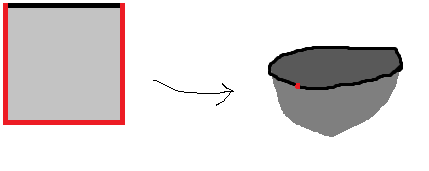
\includegraphics[]{I^2.png}
\end{figure}
\paragraph{群構造}
$n\ge 2$に対し\footnote{$n=1$だと,道の終点が$A$に含まれることしか保証されていないので,「道をつなぐ」ことが自然に定義できない.例えば$A$が2点集合だった場合を考えればわかる.},$\pi_n(X,A)$に群構造を入れる.
$f,g\colon (I^n,\partial I^n,J^n)\to (X,A,*)$に対し,その積$f\cdot g\colon (I^n,\partial I^n,J^n)\to (X,A,*)$を,\[
  (f\cdot g)(t_1,\dots,t_n):=\left\{
  \begin{alignedat}{5}
    &f(2t_1&&,t_2,\dots,t_n)\ \ &&(0&&\le t_1\le 1/2&&)\\
    &g(2t_1-1&&,t_2,\dots,t_n)\ \ &&(1/2&&\le t_1\le 1&&)
  \end{alignedat}\right.
\]と定めると,写像空間$\mathrm{Map}((I^n,\partial I^n,J^n),(X,A,*))$に$H$-spaceの構造が入る(略).よってホモトピー群に群の構造が入る.また$n\ge 3$なら$\pi_n(X,A)$はAbel群である.可換なことの証明は絶対バージョンと同様である.$n=2$だと可換とは限らないのはなぜか.$\pi_1(X)$が可換とは限らないという事実よりも非自明に思えるので,もう少しちゃんと考えたい(@TODO).$X:=(D^2\vee D^2,S^1\vee S^1)$への2種類の標準的なinclusion\ $i_1,i_2\colon(D^2,S^1)\hookrightarrow X$の積$i_1\cdot i_2$と$i_2\cdot i_1$の間に基点を止めた相対ホモトピーがなさそうなのでそれで理解できそうだが$\dots$(これこそ障害理論の適用例として使える?(2024/5/4追記 {\color{red}使えない}.普通に対のホモトピー完全列を使えば示せてしまう)).
\begin{figure}[h]
  \centering
  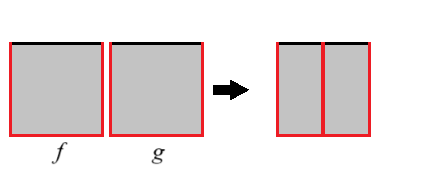
\includegraphics{defOfHomotopyGroup_composition.png}
\end{figure}

\paragraph{二つ目の定義(discを使った定義)}@TODO $I^n$を$D^n$に置き換えた場合にpinch mapおよびfoldingmapを導入し,上の定義とは少し異なる幾何学的直感を与える,しかし同一視できる群構造の入れ方を具体的に書き下しておく.
\paragraph{三つ目の定義(homotopy fiberの$n-1$次loopspaceの$0$次ホモトピー群)}@TODO loop spaceに標準的な積が定まり,それが$H$-spaceになることを述べた後$\pi_n(X,A):=\pi_0(\Omega^{n-1}(\mathrm{Path}(X,{*},A)))$と定める.
\paragraph{四つ目の定義(homotopy fiberの$n-1$次ホモトピー群)}@TODO inclusion $A\hookrightarrow X$のホモトピーファイバーの$n-1$次ホモトピー群を$n$じ相対ホモトピー群として定める.loop spaceの性質をいくつか使えば三つ目のとほぼ同じに見える.
\paragraph{すべての定義を自然に同一視できること}4つの定義によって作られた相対ホモトピー群の間に自然な同型を構成する.面倒だが,いろんな定義をinterchangeablyに使えることと,その間の同型を具体的に知っておくこと,また幾何学的に絵で理解できる定義とabstractに作られた定義の間の対応を具体的に見ておくことで,abstractな対象に対する直感ができることは重要だと思うのでやる.
\subsection{Hurewiczの定理}
\paragraph{Hurewicz homomorphism}定理に登場するHurewicz homomorphism $\rho\colon\pi_n(X,A)\to H_n(X,A)$の定義を述べる.$f\colon (D^n,S^{n-1})\to(X,A)$が$\alpha\in\pi_n(X,A)$を代表するとする\footnote{$f$は基点$*$を保つ写像だが,記法を短くするため$(D^n,S^{n-1},*)$等の「$*$」は略す.}.また,生成元$[D^n,S^{n-1}]\in H_n(D^n,S^{n-1})$を固定する.これは$(D^n,S^{n-1})$の向きを固定することと対応する.このとき,Hurewicz map $\rho\colon\pi_n(X,A)\to H_n(X,A)$を\[
  \rho(\alpha):=f_*([D^n,S^{n-1}])
\]と定める.ホモロジー論のホモトピー不変性により,この定義はwell-definedである.
\begin{lem}
  Hurewicz mapは準同型である.
\end{lem}
\begin{proof}
  ホモトピー群の定義は,二つ目のものを採用する.$f,g\colon (D^n,S^{n-1})\to (X,A)$がそれぞれ$\alpha,\beta\colon\pi_n(X,A)$を代表するとする.このとき,\begin{align*}
    \rho(\alpha\beta)&=\rho([f][g])\\
    &=\rho([(f\vee g)\circ \mathrm{pinch}])\\
    &=(f\vee g)_*\mathrm{pinch}_*(\sigma)
  \end{align*}
  である.ここで生成元$\sigma\in H_n(D^n,S^{n-1})\cong \mathbb{Z}$を一つ固定した.包含$i_1,i_2\colon (D^n,S^{n-1})\to (D^n\vee D^n,S^{n-1}\vee S^{n-1})$によりひきおこされる埋め込みにより,$H_n((D^n\vee D^n,S^{n-1}\vee S^{n-1}))\cong \mathbb{Z}\oplus \mathbb{Z}$の生成系$\sigma_1:=i_{1*}\sigma,\ \sigma_{2}:=i_{2*}\sigma$を得る.$\mathrm{pinch}_*(\sigma)=\pm\sigma_1\pm\sigma_2$となる(複号は$\mathrm{pinch}$のとりかたによる).よって,\begin{align*}
    \rho(\alpha\beta)&=(f\vee g)_*(\pm\sigma_1\pm\sigma_2)\\
    &=\pm(f\vee g)_*i_{1*}\sigma\pm(f\vee g)_*i_{2*}\sigma\\
    &=\pm((f\vee g)\circ i_1)_*\sigma\pm((f\vee g)\circ i_2)_*\sigma\\
    &=\pm f_*\sigma\pm g_*\sigma\\
    &=\rho(\alpha)+\rho(\beta)
  \end{align*}
  である\footnote{4つ目の等号は,$(f\vee g)\circ i_1=f$などから従う.$f\vee g$はウェッジ和の普遍性により引き起こされた写像なので,可換図式を追えばこのことは示せる.}.
\end{proof}
\subsection{Freudenthalの懸垂定理}
\subsection{Whiteheadの定理}
\section{局所係数の(コ)ホモロジー}
\subsection{局所系の2種類の定義}
\subsection{局所係数の(コ)ホモロジーの計算例}
\section{障害理論}
\subsection{CW複体上の写像を延ばせるかどうかのcriterion}
\subsubsection{Obstruction Cocycle}
$(X,A)$を相対CW-複体,$Y$を単連結な位相空間,$n\ge 0$とする.このとき,$n$-skeleton $X^{(n)}$上の連続写像$f_n\colon X^{(n)}\to Y$を$n+1$-skeleton $X^{(n+1)}$上に連続に延ばせるかという問題を考える.$(n+1)$-cell全体を$\{e_{\lambda}\}_{\lambda\in \Lambda_{n+1}}$とおき,各$\lambda\in\Lambda_{n+1}$に対し特性写像$\varphi_\lambda\colon (D^{n+1}_\lambda,S^n_\lambda)\to (X^{(n+1)},X^{(n)})$を固定する.

この状況において,$f_n$が$e_\lambda$に延びることは$f_n\circ\varphi_\lambda|_{S^n_\lambda}\colon S^n_\lambda\to Y$がnull-homotopicであることと等しく,また$\Leftrightarrow$ $[f_n\circ \varphi_\lambda|_{S^n_\lambda}]=0\in \pi_n(Y)$であることと等しい.したがって$f_n$が$X^{(n+1)}$に延びるための条件は,任意の$\lambda\in\Lambda_{n+1}$に対して,$[f_n\circ \varphi_\lambda|_{S^n_\lambda}]=0\in \pi_n(Y)$となることである.

以上の構成により定まる写像$\Lambda_{n+1}\to \pi_n(Y)$は$X$のcellular cochain $\tilde{\mathcal{O}}(f_n)\in C^{n+1}(X,A;\pi_n(Y))=\Hom_\mathbb{Z}(C_{n+1}(X,A),\pi_n(Y))$を定める.

\begin{prop}
  $\tilde{\mathcal{O}}(f_n)$は特性写像$\{\varphi_\lambda\}_{\lambda\in\Lambda_{n+1}}$のとりかたに依らない.
\end{prop}
\begin{proof}
  次の図式を使って$\tilde{\mathcal{O}}(f_n)$の構成を丁寧にみる.ここで,$\rho$は生成元$[D^n,S^{n-1}]\in H_n(D^n,S^{n-1})$を固定して定められたHurewicz準同型である.また,左下の$\rho$が同型だった場合のみ考える\footnote{$X^{(n)}$が単連結なら$\rho$は同型だが,そうでない場合は基本群の作用で相対ホモトピー群を割ったものから生える$\bar{\rho}$が同型になる.この場合でも同様にobstruction cochainを構成できる.\cite{whitehead2012elements}のV-5(p. 229)を参照.}.\[
  \xymatrix{
    &\bigoplus_\lambda\pi_n(S^n_\lambda)\ar[ld]_{\bigoplus_\lambda(\varphi_\lambda|_{S^n_\lambda})_*}\ar[rd]^{\bigoplus_\lambda\rho}_{\cong}&\\
    \pi_n(X^{(n)})\ar[r]^\rho & 
    H_n(X^{(n)})  & 
    \bigoplus_\lambda H_n(S^n_\lambda)\ar[l]^{\bigoplus_\lambda(\varphi_\lambda|_{S^n_\lambda})_*}\\
    \pi_{n+1}(X^{(n+1)},X^{(n)})\ar[u]^{\partial}\ar[r]_\rho^{\cong} & 
    H_{n+1}(X^{(n+1)},X^{(n)})\ar[u]^\partial & 
    \bigoplus_\lambda H_{n+1}(D^{n+1}_\lambda,S^n_\lambda)\ar[u]_\partial^\cong\ar[l]^{\bigoplus_\lambda (\varphi_\lambda)_*}_\cong
  }\]
  $\tilde{\mathcal{O}}(f_n)$とは何かというと,各$[D^{n+1}_\lambda,S^{n}_\lambda]\in H_{n+1}(D^{n+1}_\lambda,S^{n}_\lambda)$に対し$[\varphi_\lambda|_{S^n_\lambda}]=(\varphi_\lambda|_{S^n_\lambda})_*[\id_{S^n_\lambda}]$(最上段左の矢印による像)を対応させて準同型$\bigoplus_\lambda H_{n+1}(D^{n+1}_\lambda,S^n_\lambda)\to \pi_n(X_n)$をつくり,さらに最初に固定していた特性写像により定まる同型(最下段右の矢印)で引き戻した準同型を$(f_n)_*$で$\pi_n(Y)$に押し出してできた準同型のことである.$(f_n)_*$で押し出す前の準同型$H_{n+1}(X^{(n+1)},X^{(n)})\to \pi_n(X^{(n)})$が特性写像のとりかたに依らないことを示せばよい.

  まず$H_{n+1}(D^{n+1}_\lambda,S^n_\lambda)$の元をとっておきながら最上段左の矢印による像を対応させてしまっているので,自然なやり方で$H_{n+1}(D^{n+1}_\lambda,S^n_\lambda)$と$\pi_n(S^n_\lambda)$の間の写像を作らないといけない.そこで作られたのが上の図式である.上と左の四角はHurewicz準同型が対のホモロジー完全列とホモトピー完全列の間の図式の準同型になっていることから,また,右の四角は対のホモトピー完全列の連結準同型の自然性から可換である.

  右下からスタートして基本類を移した元$\rho_\lambda\partial[D^{n+1}_\lambda,S^n_\lambda]$が$\id_{S^n\lambda}$に等しいことを示せば最下段真ん中からスタートして反時計回りに図式を大回りして$\pi_n(X^{(n)})$へ至る矢印を$(f_n)_*$で押し出したものと$\tilde{\mathcal{O}}(f_n)$が等しいことが言えて,図式の可換性からそれは$(f_n)_*\circ\partial\circ\rho^{-1}$に等しく,これは特性写像のとりかたに依らないことまでわかる.
\end{proof}

\begin{prop}
  $\tilde{\mathcal{O}}(f_n)$はコサイクルである.
\end{prop}
\begin{proof}
  次の図式をみる.
  \[\xymatrix{\pi_{n+2}(X^{(n+2)},X^{(n+1)})\ar[r]^{\rho}_\cong\ar[d]_\partial& H_{n+2}(X^{(n+2)},X^{(n+1)})\ar[dd]^{\partial^\mathrm{cell}}\\
  \pi_{n+1}(X^{(n+1)})\ar[d]_{i_*}&\\
  \pi_{n+1}(X^{(n+1)},X^{(n)})\ar[r]^\rho_\cong\ar[d]_\partial&H_{n+1}(X^{(n+1)},X^{(n)})\ar[ld]\\
  \pi_n(X^{(n)})&}
  \]
  上半分は$\partial^\mathrm{cell}$の定義より可換である.また右下の矢印の後ろに$(f_n)_*$を合成したものが$\tilde{\mathcal O}(f_n)$である.$\delta \tilde{\mathcal O}(f_n)=\tilde{\mathcal{O}}(f_n)\circ\partial^\mathrm{cell}$だが,図式が可換であることおよび$\partial\circ i_*=0$ゆえ,$\delta\tilde{\mathcal O}(f_n)=0$である.
\end{proof}
$\tilde{\mathcal{O}}(f_n)$をコホモロジー類に落としたものを$\mathcal{O}(f_n)$
とかく.

\subsubsection{Difference Cochain}
単位区間$I$に標準的な胞体分割$I=\{0\}\cup \Int I\cup\{1\}$を与えておく.

$f,g\colon X^{(n)}\to Y$,$f|_{X^{(n-1)}}$と$g|_{X^{(n-1)}}$をつなぐホモトピー$G\colon I\times X^{(n-1)}\to Y$が与えられたとする.このとき写像\index{Ffg@$F_{f,g}$}
\[
  F_{f,g}\colon (I\times X)^{(n)}=\{0,1\}\times X^{(n)}\cup\Int I\times X^{(n-1)}\to Y
\]
が$0\times X^{(n)}$上で$f$,$1\times X^{(n)}$上で$g$,$I\times X^{(n-1)}$上で$G$とすると定まる.このとき,$(f,g)$の$G$に関する\index{diffeence cochain}difference cochain $d(f,G,g)\in C^n(X,A;\pi_n(Y))$を,各$n$-cell $e$に対し,
\[
  d(f,G,g)(e):=\tilde{\mathcal{O}}(F_{f,g})(\Int I\times e)
\]
で定める.特別に$f|_{X^{(n-1)}}=g|_{X^{(n-1)}}$かつ$G$が定置のとき$d_{f,g}:=d(f,G,g)$とかく.

\begin{prop}
  (difference cochainはホモトピーの延長を見つける)上の状況で$d(f,G,g)=0$であることと,ホモトピー$G$が$I\times X^{(n)}$に延びることは同値である.
\end{prop}
\begin{proof}
  まず,$I\times X^{(n-1)}\cup \{0,1\}\times X^{(n)}=(I\times X^{(n)})^{(n)}$ゆえ,$F_{f,g}$が$I\times X^{(n)}$に延びることは$\tilde{\mathcal{O}}(F_{f,g})=0\in C^{n+1}(I\times X^{(n)},I\times X^{(n-1)}\cup \{0,1\}\times X^{(n)};\pi_n(Y))$と同値であることに注意する.

  $d(f,G,g)=0$とする.$I\times X^{(n)}$の$(n+1)$-cell $\Int I\times e$($e$は$X$の$n$-cell)に対し,$\tilde{\mathcal{O}}(F_{f,g})(\Int I\times e)=d(f,G,g)(e)=0$である.$I\times X^{(n)}$の$(n+1)$-cellはすべて$\Int I\times e$の形であるから$\tilde{\mathcal{O}}(F_{f,g})=0$である.

  $\tilde{\mathcal{O}}(F_{f,g})=0$とする.$X$の$n$-cell $e$を任意にとると$\Int I\times e$は$I\times X^{(n)}$の$(n+1)$-cellだから$d(f,G,g)(e)=\tilde{\mathcal{O}}(F_{f,g})(\Int I\times e)=0$ゆえ$d(f,G,g)=0$である.
\end{proof}

次の補題は$f\colon X^{(n)}\to Y$が与えられたとき,それとホモトピック rel. $X^{(n-1)}$な写像$g$をうまくとることで$C^n(X,A;\pi_n(Y))$の任意の元を表すことができるということを主張している.

\label{representN-CochainAsDiffCochain}
\begin{lem}(任意の$n$-cochainはdifference cochainで表せる) $f\colon X^{(n)}\to Y$, $d\in C^n(X,A;\pi_n(Y))$とするこ.このとき$X^{(n-1)}$上で$f$と一致する$g\colon X^{(n)}\to Y$で$d_{f,g}=d$となるようなものが存在する.
\end{lem}
\begin{proof}
  (証明の気持ち)$d_{f,g}$は各$n$-cellに対して,$f\circ\varphi,g\circ\varphi$を球面$S^n$上で貼り合わせたもののホモトピー類が対応するように作るので,それが$d$に一致するようにするためには球面$S^n$の下半分を$f\circ\varphi$の定義域として使い,HEPを使って$\alpha$とホモトピックな写像になるように$S^n$上に延ばす.そうして伸ばした写像のうち$S^n$の上半分を使っているものを$g$とおく.\\


  $g|_{X^{(n-1)}}=f|_{X^{(n-1)}}$だから,あとは各$n$-cell $e$上に$g$をのばす.特性写像$\varphi\colon(D^n,S^{n-1})\to (X^{(n)},X^{(n-1)})$を固定して,$d(e)=[\alpha]$なる$\alpha\colon (S^n,*)\to (Y,*)$をとる.ここで,球面は二つの閉球を赤道で張り合わせたもの$S^n=D^n_1\cup_{S^{n-1}}D^n_2$とみなす.

  $f\circ \varphi\colon D^n_2\to Y$と$\alpha|_{D^n_2}$はnull-homotopicなので,$\alpha|_{D^n_2}$を$f\circ \varphi$につなぐホモトピー$h\colon D^n_2\to Y^I$がある.対$(S^n,D^n_2)$のHEPより,$h$は$\tilde{h}\colon S^n\to Y^I$に延びる.\[
  \xymatrix{
    D^n_2 \ar[r]^h \ar@{^{(}->}[d]
    & Y^I \ar[d]^{\mathrm{ev}_0}\\
    S^n \ar[r]_{\alpha} \ar@{.>}[ru]_{\tilde{h}}
    & Y
  }
  \]
  $e$上での$g$を合成\[
    D^n_1\hookrightarrow S^n\xrightarrow{\tilde{h}}Y^I\xrightarrow{\mathrm{ev}_1}Y  
  \]と定める.これが実際に$d_{f,g}=d$を与えることを示す.

  $n$-cell $e$を任意にとる.このとき,$d_{f,g}(e)=[\mathrm{ev}_1\circ\tilde{h}]=[\alpha]=d(e)$である.一つ目のイコールは$h$の定義と$g$の定義による.2つ目のイコールは上の図式の右下の三角形が可換であることと$\alpha=\tilde{h}(\cdot)(0)\sim\tilde{h}(\cdot)(1)=\mathrm{ev}_1\circ \tilde{h}$からいえる.
\end{proof}

\begin{lem}
  $\delta d(f,G,g)=\tilde{\mathcal{O}}(g)-\tilde{\mathcal{O}}(f)$
\end{lem}
\begin{proof}
$d:=d(f,G,g)$,$F:=F_{f,g}$とかく.

  各$e\in C_{n+1}(X,A)$に対し,\begin{align*}
    \delta d(e)&=d(\partial e)\\
    &=\tilde{\mathcal{O}}(F)(\Int I\times \partial e)
  \end{align*}
  である.ここで,$\tilde{\mathcal{O}}(F)$はcocycleゆえ,\begin{align*}
    0&=\delta\tilde{\mathcal{O}}(F)(\Int I\times e)\\
    &=\tilde{\mathcal{O}}(F)(\partial(\Int I\times e))\\
    &=\tilde{\mathcal{O}}(F)(1\times e-0\times e-\Int I\times \partial e)
  \end{align*}である.したがって,$e$の特性写像$\varphi$を一つ固定すると,\begin{align*}
    \delta d(e)&=\tilde{\mathcal{O}}(F)(1\times e)-\tilde{\mathcal{O}}(F)(0\times e)\\
    &=[g\circ\varphi|{S^n}]-[f\circ\varphi|{S^n}]\\
    &=\tilde{\mathcal{O}}(g)(e)-\tilde{\mathcal{O}}(f)(e)
  \end{align*}である.
\end{proof}

\subsubsection{コホモロジーのレベルでのobstruction}
次の命題は,$X^{(n)}$上に延ばせる$X^{(n-1)}$上の写像がさらに$X^{(n+1)}$に延ばせる条件をコホモロジーの言葉で述べる.
\begin{prop}
  $f_n\colon X^{(n)}\to Y$に対し,\[
    \mathcal{O}(f_n)=0\Leftrightarrow f_n|_{X^{(n-1)}}が(X^{(n)}-X^{(n-1)}上でfと異なるかもしれないが,)X^{(n+1)}上に延びる.
  \]である.
\end{prop}
\begin{proof}
  $\mathcal{O}(f_n)=0$とする.このときある$d\in C^{n}(X,A;\pi_{n}(Y))$が存在して,$\delta d=\tilde{\mathcal{O}}(f_n)$である.$X^{(n-1)}$上で$f_n$と一致する$g\colon X^{(n)}\to Y$を$d_{f_n,g}=-d$となるようにとる.$\tilde{\mathcal{O}}(g)=\delta d_{f_n,g}+\tilde{\mathcal{O}}(f_n)=\tilde{\mathcal{O}}(f_n)-\delta d=0$である.よって$g$は$X^{(n+1)}$に延びる.\\

  逆に,$g\colon X^{(n)}\to Y$が$X^{(n-1)}$上で$f_n$と一致し,$X^{(n+1)}$に延びるとする.このとき$\tilde{\mathcal{O}}(g)=0$で,$\tilde{\mathcal{O}}(f_n)=\tilde{\mathcal{O}}(f_n)-\tilde{\mathcal{O}}(g)=-\delta d_{f_n,g}$ゆえ$\mathcal{O}(f_n)=0$である.
\end{proof}
\subsubsection{ホモトピーを延ばすときのobstruction}

ホモトピーを延ばす時のobstructionはコホモロジーのレベルではどう書かれるか.相対CW-複体$(X,A)$に対し,$(\hat{X},\hat{A}):=(I,\partial I)\times(X,A)=(I\times X,\partial I\times X\cup I\times A)$とおく.$f,g\colon X\to Y$と$f|_{X^{(n-1)}}$を$g|_{X^{(n-1)}}$につなぐ$A$-ホモトピー$H\colon I\times X^{(n-1)}\to Y$が与えられたとする.このとき写像$F_{f,g}\colon \hat{X}^{(n)}\to Y$\footnote{$\hat{X}^{(n)}=\partial I\times X\cup I\times X^{(n-1)}$である.}が定まる.これが$\hat{X}^{(n+1)}$に延びる,すなわちホモトピー$H$が$I\times X^{(n)}$に延びるためのobstruction cocycle $\tilde{\mathcal{O}}(F_{f,g})\in C^{n+1}(\hat{X},\hat{A};\pi_n(Y))$が定まる.
\begin{cor}
  上の状況で$d(f,H,g)$はcocycleである.またそのコホモロジー類$D(f,H,g)\in H^{n}(X,A;\pi_n(Y))$が0であることは$H|_{I\times X^{(n-1)}}$が$I\times X^{(n+1)}$に延びることと同値である.
\end{cor}
\begin{proof}
  まず,$f,g$はずでに$X^{(n+1)}$に延びているので,$\delta d(f|_{X^{(n)}},H,g|_{X^{(n)}})=\tilde{\mathcal{O}}(g|_{X^{(n)}})-\tilde{\mathcal{O}}(f|_{X^{(n)}})=0$である.

  上の命題より,$\mathcal{O}(F_{f,g})=0$であることと$F_{f,g}$の$\{0,1\}\times X\cup I\times X^{(n+1)}$への延長$\tilde{F}$が($F_{f,g}$とは$I\times (X^{(n)}-X^{(n-1)})$上で異なるかもしれないが)存在することは同値である.

  $\mathcal{O}(F_{f,g})$と$D(f,H,g)$の対応を作る.3対$(I\times ,\partial I\times X\cup I\times A,1\times X\cup I\times A)$のホモロジー完全列\[
    \leftarrow H^p(\partial I\times X\cup I\times A,1\times X\cup I\times A)
    \leftarrow H^p(I\times X,1\times X\cup I\times A)
    \leftarrow H^p(I\times X,\partial I\times X\cup I\times A)
    \leftarrow
  \]
  を見る.HEPにより,$I\times X$は$1\times X\cup I\times A$にレトラクトするので,$H^p(I\times X,1\times X\cup I\times A)$は$p>0$で$0$である.よって,$p>0$に対し連結準同型は同型
  \[
    H^{p+1}(I\times X,\partial I\times X\cup I\times A)
    \leftarrow H^p(\partial I\times X\cup I\times A,1\times X\cup I\times A)
  \]
  を与える.さらに,inclusion
  \[
    i\colon (0\times X,0\times A)\rightarrow (\partial I\times X\cup I\times A,1\times X\cup I\times A)
  \]
  が引き起こすコホモロジーの同型\footnote{両方の部分空間の方をつぶすと,ともに$X/A$になる}を合成すると自然な同型
  \[
    \partial^*\circ (i^*)^{-1}\colon H^p(X,A)\to H^{p+1}(\hat{X},\hat{A})
  \]
  を得る.

  上の同型が対応$D(f,H,g)\mapsto \mathcal{O}(F_{f,g})$を与えることを見る({\color{red}まだ示せてない!}).
\end{proof}
\subsection{E-M空間}

\bibliographystyle{alpha}
\bibliography{bib}

\printindex

\end{document}